\chapter{Filtro Pasa-Altos Activo de 4to Orden (Chebyshev MFB)}
\label{sec.ej3:filtro_hpf}

\section{Especificaciones y Topología Circuital}
\label{sec.ej3:especificaciones}

El segundo diseño asignado por la cátedra consiste en un filtro pasa-altos de cuarto orden con aproximación Chebyshev,
cuyas especificaciones son:
\begin{itemize}
    \item \textbf{Orden del filtro:} $n = 4$, conformado por dos etapas de realimentación múltiple (MFB) en cascada.
    \item \textbf{Aproximación matemática:} Chebyshev de 4to orden con rizado en banda de paso de $A_{\max} = 3 \unit{\decibel}$.
    \item \textbf{Frecuencia límite de banda de paso:} $f_p = 11.0 \unit{\kilo\hertz}$.
    \item \textbf{Ganancia total en banda de paso:} $A_v = 6.00 \unit{\volt\per\volt} \implies 20\log_{10}(6) \approx +15.56 \unit{\decibel}$.
    \item \textbf{Topología circuital:} Realimentación múltiple (MFB, Multiple Feedback / Rauch), diseñada de acuerdo
    con los métodos de Pactitis y la documentación de aplicación de Texas Instruments (SLOA088).
    \item \textbf{Estado de ejecución:} Implementado físicamente y ensayado en laboratorio.
\end{itemize}

\section{Deducción Analítica de la Celda MFB Pasa-Altos}
\label{sec.ej3:deduccion_mfb}

La topología MFB pasa-altos es una estructura inversora que emplea tres capacitores ($C_1, C_2, C_3$) y dos
resistencias ($R_1, R_2$) por celda de segundo orden.

El análisis nodal en pequeña señal sobre la celda se formula de la siguiente manera:
\begin{enumerate}
    \item La entrada $V_i$ ingresa a través de $C_1$ a un nodo intermedio $V_1$. Dicho nodo se encuentra conectado a:
    $C_1$ desde la entrada, $R_1$ hacia la referencia de masa virtual, $C_2$ hacia el terminal de salida $V_o$, y
    $C_3$ hacia la entrada inversora del amplificador operacional ($V_-$).
    \begin{equation}
    \label{eq.ej3:kcl_nodo1}
    (V_1 - V_i) s C_1 + \frac{V_1}{R_1} + (V_1 - V_o) s C_2 + (V_1 - V_-) s C_3 = 0
    \end{equation}
    \item En la entrada inversora del amplificador operacional, el nodo suma las corrientes provenientes de $C_3$ y de
    la resistencia de realimentación $R_2$ conectada a la salida:
    \begin{equation*}
    (V_- - V_1) s C_3 + \frac{V_- - V_o}{R_2} = 0
    \end{equation*}
    \item Dado que la entrada no inversora se fija a la tensión de referencia ($V_+ = 0$), el cortocircuito virtual
    impone $V_- = 0$. Despejando $V_1$ de la ecuación de la entrada inversora:
    \begin{equation}
    \label{eq.ej3:v1_despeje}
    - V_1 s C_3 - \frac{V_o}{R_2} = 0 \implies V_1 = - \frac{V_o}{s R_2 C_3}
    \end{equation}
    \item Sustituyendo $V_1$ en la ecuación del nodo intermedio y multiplicando miembro a miembro por $-s R_2 C_3$:
    \begin{equation*}
    V_o \left[ s(C_1 + C_2 + C_3) + \frac{1}{R_1} \right] = - s^2 R_2 C_1 C_3 V_i - s^2 R_2 C_2 C_3 V_o
    \end{equation*}
\end{enumerate}

Reordenando términos y dividiendo por el coeficiente cuadrático $R_2 C_2 C_3$, se obtiene la función de transferencia
canónica de segundo orden de la celda MFB pasa-altos:
\begin{equation}
\label{eq.ej3:transferencia_mfb}
H_{\text{MFB}}(s) = \frac{V_o(s)}{V_i(s)} = \frac{- \left(\frac{C_1}{C_2}\right) s^2}{s^2 + s \left[ \frac{C_1 + C_2 + C_3}{R_2 C_2 C_3} \right] + \frac{1}{R_1 R_2 C_2 C_3}}
\end{equation}

De la Ecuación~(\ref{eq.ej3:transferencia_mfb}) se deducen directamente los parámetros canónicos:
\begin{itemize}
    \item \textbf{Ganancia asintótica en alta frecuencia ($s \to \infty$):}
    \begin{equation}
    \label{eq.ej3:kinf}
    K_\infty = - \frac{C_1}{C_2}
    \end{equation}
    \item \textbf{Pulsación natural resonante ($\omega_0$):}
    \begin{equation}
    \label{eq.ej3:w0_mfb}
    \omega_0 = \frac{1}{\sqrt{R_1 R_2 C_2 C_3}}
    \end{equation}
    \item \textbf{Factor de amortiguamiento y calidad ($Q$):}
    \begin{equation}
    \label{eq.ej3:q_mfb}
    \frac{\omega_0}{Q} = \frac{C_1 + C_2 + C_3}{R_2 C_2 C_3} \implies Q = \frac{\sqrt{R_2 / R_1}}{\frac{C_1 + C_2 + C_3}{\sqrt{C_2 C_3}}}
    \end{equation}
\end{itemize}

\section{Síntesis de Chebyshev y Distribución de Etapas}
\label{sec.ej3:sintesis}

Para una aproximación Chebyshev de 4to orden con rizado de $A_{\max} = 3 \unit{\decibel}$, el polinomio denominador
en el dominio normalizado pasa-bajos presenta polos con factores de calidad marcadamente dispares: una sección de
baja $Q$ ($Q \approx 1.08$) y una sección fuertemente resonante ($Q \approx 3.56$).

Mediante la transformación estándar en frecuencia pasa-bajos a pasa-altos ($s_n \to \omega_p / s$), los polos se
invierten en frecuencia respecto a $\omega_p = 2\pi \times 11.0 \unit{\kilo\hertz} \approx 69115 \unit{\radian\per\second}$.
Siguiendo las pautas de Texas Instruments y Pactitis, la primera etapa asume la función moderadamente selectiva con
menor ganancia, y la segunda etapa implementa el polo más resonante.

\subsection{Polarización Unipolar con Masa Virtual (+12 V)}
Dado que el circuito se alimenta con fuente simple de $+24 \unit{\volt}$, la señal senoidal de entrada requiere una
referencia de reposo simétrica para admitir excursiones positivas y negativas sin recorte.

Para ello, se implementó una red de masa virtual (GNDA) a partir de un divisor resistivo simétrico de
$R_3 = 10 \unit{\kilo\ohm}$ y $R_4 = 10 \unit{\kilo\ohm}$ conectado entre $+24 \unit{\volt}$ y GND, desacoplado
mediante un capacitor de $100 \unit{\nano\farad}$ y asistido por una sección del amplificador operacional LM324
configurada como seguidor de tensión. Este nodo de $+12 \unit{\volt}$ alimenta las entradas no inversoras de las dos
celdas de filtrado y el retorno del resistor $R_1$, aislando dinámicamente las etapas de la fuente principal.

\subsection{Selección y Ajuste de Componentes Comerciales}
Para satisfacer la ganancia global requerida de $A_v = 6.00 \unit{\volt\per\volt}$ ($+15.56 \unit{\decibel}$):
\begin{enumerate}
    \item \textbf{Etapa 1:}
    Se adoptaron capacitores de entrada y acoplo inversor normalizados $C_1 = 1.0 \unit{\nano\farad}$ y
    $C_3 = 1.0 \unit{\nano\farad}$. A fin de ajustar la ganancia individual a $K_{\infty 1} \approx 3.0 \unit{\volt\per\volt}$,
    el capacitor de realimentación $C_2$ se conformó conectando en paralelo dos capacitores cerámicos comerciales:
    $C_2 = 180 \unit{\pico\farad}$ y $C_7 = 150 \unit{\pico\farad}$, logrando una capacidad efectiva de
    $C_{2,\text{eq}} = 330 \unit{\pico\farad}$.
    \begin{equation*}
    K_{\infty 1} = - \frac{C_1}{C_{2,\text{eq}}} = - \frac{1000 \unit{\pico\farad}}{330 \unit{\pico\farad}} = -3.03 \unit{\volt\per\volt}
    \end{equation*}
    Con $R_1 = 8.0 \unit{\kilo\ohm}$ y $R_2 = 47.0 \unit{\kilo\ohm}$, los parámetros de la celda resultan:
    \begin{equation*}
    f_{01} = \frac{1}{2\pi\sqrt{8\text{k} \cdot 47\text{k} \cdot 330\text{p} \cdot 1\text{n}}} = 14.29 \unit{\kilo\hertz}, \qquad Q_1 \approx 0.60
    \end{equation*}

    \item \textbf{Etapa 2:}
    Se adoptaron $C_4 = 1.0 \unit{\nano\farad}$, $C_5 = 470 \unit{\pico\farad}$ y $C_6 = 1.0 \unit{\nano\farad}$.
    La ganancia de la etapa resulta:
    \begin{equation*}
    K_{\infty 2} = - \frac{C_4}{C_5} = - \frac{1000 \unit{\pico\farad}}{470 \unit{\pico\farad}} = -2.13 \unit{\volt\per\volt}
    \end{equation*}
    Con $R_5 = 3.0 \unit{\kilo\ohm}$ y $R_6 = 180.0 \unit{\kilo\ohm}$, se obtienen:
    \begin{equation*}
    f_{02} = \frac{1}{2\pi\sqrt{3\text{k} \cdot 180\text{k} \cdot 470\text{p} \cdot 1\text{n}}} = 9.99 \unit{\kilo\hertz}, \qquad Q_2 \approx 2.15
    \end{equation*}
\end{enumerate}

La ganancia global asintótica en la banda de paso resulta:
\begin{equation}
\label{eq.ej3:ganancia_total_calc}
A_{v,\text{total}} = K_{\infty 1} \cdot K_{\infty 2} = (-3.03) \times (-2.13) = +6.45 \unit{\volt\per\volt} \implies +16.19 \unit{\decibel}
\end{equation}
presentando un desvío de apenas $+0.63 \unit{\decibel}$ respecto al valor nominal de $+15.56 \unit{\decibel}$, plenamente
compensable por las pérdidas parásitas en circuito impreso.

\begin{figure}[!ht]
\centering
\begin{circuitikz}[american, scale=0.74, transform shape]
    % ==================== ETAPA 1 ====================
    \draw (0,0) node[left] {$V_{\text{in}}$} to[short, o-] (0.8,0)
          to[C, l=$C_1$, a=\SI{1}{\nano\farad}] (2.8,0) coordinate(n1);
    \draw (2.8,0) to[R, l=$R_1$, a=\SI{8}{\kilo\ohm}] (2.8, -2.5) to[short] (2.8, -2.8) node[ground] {};
    \draw (n1) to[C, l=$C_3$, a=\SI{1}{\nano\farad}] (5.2, 0) coordinate(nin1);
    \draw (7.0, -0.5) node[op amp] (oa1) {};
    \node[font=\footnotesize] at ($(oa1.center)+(0.15,0)$) {$U_{1A}$};
    \draw (nin1) -- (oa1.-);
    \draw (oa1.+) -- (5.8, -1.0) node[ground] {};
    
    \draw (nin1) -- (5.2, 1.5) to[C, l=$C_2$, a=\SI{180}{\pico\farad}] (8.5, 1.5) -- (8.5, -0.5) coordinate(out1);
    \draw (n1) -- (2.8, 3.4) to[R, l=$R_2$, a=\SI{47}{\kilo\ohm}] (9.3, 3.4) -- (9.3, -0.5);
    \draw (oa1.out) -- (9.3, -0.5);
    
    % ==================== ETAPA 2 ====================
    \draw (9.3, -0.5) to[short] (10.5, -0.5)
          to[C, l=$C_4$, a=\SI{1}{\nano\farad}] (12.5, -0.5) coordinate(n2);
    \draw (12.5, -0.5) to[R, l=$R_5$, a=\SI{3}{\kilo\ohm}] (12.5, -3.0) to[short] (12.5, -3.3) node[ground] {};
    \draw (n2) to[C, l=$C_6$, a=\SI{1}{\nano\farad}] (14.9, -0.5) coordinate(nin2);
    \draw (16.7, -1.0) node[op amp] (oa2) {};
    \node[font=\footnotesize] at ($(oa2.center)+(0.15,0)$) {$U_{1B}$};
    \draw (nin2) -- (oa2.-);
    \draw (oa2.+) -- (15.5, -1.5) node[ground] {};
    
    \draw (nin2) -- (14.9, 1.0) to[C, l=$C_5$, a=\SI{470}{\pico\farad}] (18.2, 1.0) -- (18.2, -1.0) coordinate(out2);
    \draw (n2) -- (12.5, 3.0) to[R, l=$R_6$, a=\SI{180}{\kilo\ohm}] (19.0, 3.0) -- (19.0, -1.0);
    \draw (oa2.out) -- (19.0, -1.0) to[short, -o] (20.0, -1.0) node[right] {$V_{\text{out}}$};
\end{circuitikz}
\caption{Diagrama circuital del filtro activo pasa-altos MFB de 4to orden (Chebyshev $3\,\text{dB}$, $K=6\,\text{V/V}$).}
\label{fig.ej3:sch}
\end{figure}

\section{Simulación y Ensayos de Laboratorio}
\label{sec.ej3:resultados}

Se simuló en SPICE la respuesta en frecuencia del filtro pasa-altos MFB
(\texttt{filter-HP-MFB-ac.csv}). La curva Bode resultante (Figura~\ref{fig.ej3:bode_ac}) refleja los parámetros
de la aproximación Chebyshev:
\begin{itemize}
    \item Ganancia en la banda de paso superior de $+15.56 \unit{\decibel}$ ($6.00 \unit{\volt\per\volt}$), verificando la meseta de alta frecuencia.
    \item Frecuencia de corte nominal en $f_p = 11.0 \unit{\kilo\hertz}$, donde la magnitud alcanza la cota inferior de rizado ($+15.56 \unit{\decibel}$).
    \item Sobreelevación característica de Chebyshev en la zona de borde ($11\text{--}15 \unit{\kilo\hertz}$) contenida dentro del rizado $A_{\max} = 3 \unit{\decibel}$.
    \item Pendiente asintótica en la banda atenuada de $+80 \unit{\decibel\per\decade}$ por debajo de $8 \unit{\kilo\hertz}$, proporcionando un rechazo profundo frente a componentes de baja frecuencia.
\end{itemize}

\begin{figure}[!ht]
\centering
\begin{tikzpicture}
  \begin{axis}[
    width=0.95\textwidth,
    height=7.5cm,
    xmode=log,
    xmin=500, xmax=500000,
    ymin=-40, ymax=25,
    ytick={-40, -20, 0, 10, 20},
    grid=both,
    grid style={line width=.1pt, draw=gray!25},
    major grid style={line width=.2pt, draw=gray!45},
    xlabel={Frecuencia [\unit{\hertz}]},
    ylabel={Ganancia $|A_v|$ [\unit{\decibel}]},
    legend style={at={(0.03,0.06)}, anchor=south west, font=\footnotesize}
  ]
    % Ganancia simulada
    \addplot[very thick, color=blue!85!black] table [x=freq, y=gain_db] {sources/data/data_bode_hpf.txt};
    \addlegendentry{Respuesta simulada $|A_v(f)|$}

    % Linea de ganancia asintotica
    \draw[dashed, color=gray!80!black] (axis cs:500, 16.19) -- (axis cs:500000, 16.19);
    \node[anchor=south east, font=\scriptsize, text=gray!80!black, fill=white, fill opacity=0.85, text opacity=1, inner sep=1.5pt] 
      at (axis cs:400000, 17.0) {$A_{v,\infty} = \SI{16.19}{\decibel}$};

    % Linea de nivel de rizado / -3 dB
    \draw[dotted, thick, color=red!80!black] (axis cs:500, 13.19) -- (axis cs:500000, 13.19);
    \node[anchor=south east, font=\scriptsize, text=red!80!black, fill=white, fill opacity=0.85, text opacity=1, inner sep=1.5pt] 
      at (axis cs:400000, 11.2) {Cota rizado $-\SI{3}{\decibel}$ ($\SI{13.19}{\decibel}$)};

    % Frecuencia de corte fp = 11 kHz (dato y punto -3 dB)
    \draw[dotted, thick, color=red!80!black] (axis cs:11000, -40) -- (axis cs:11000, 13.19)
      node[pos=0.35, right=2pt, font=\scriptsize, text=red!80!black, fill=white, fill opacity=0.85, text opacity=1, inner sep=1.5pt] {$f_p = \SI{11.0}{\kilo\hertz}$ (dato, $-\SI{3}{\decibel}$)};
    \addplot[only marks, mark=*, mark size=2.2pt, color=red!80!black] coordinates {(11000, 13.19)};
  \end{axis}
\end{tikzpicture}

\caption{Simulación de respuesta en frecuencia (magnitud) del filtro pasa-altos MFB de 4to orden.}
\label{fig.ej3:bode_ac}
\end{figure}

\subsection{Mediciones Temporales y Espectrales en Osciloscopio}
El filtro pasa-altos fue montado en su respectiva placa de circuito impreso (Figura~\ref{fig.ej3:placa}) y ensayado
con instrumental del laboratorio:

\begin{figure}[!ht]
\centering
\begin{subfigure}[t]{0.48\textwidth}
    \centering
    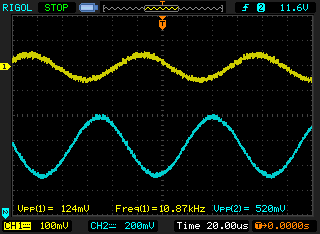
\includegraphics[width=\textwidth]{hpf_osc_11khz.png}
    \caption{Respuesta temporal en el borde de banda ($f = 10.87\,\mathrm{kHz}$): entrada $V_{\text{pp}} = 124\,\mathrm{mV}$ (amarillo), salida $V_{\text{pp}} = 520\,\mathrm{mV}$ (cian), ganancia $A_v = 4.19\,\mathrm{V/V}$ (caída de $3.3\,\mathrm{dB}$ respecto a la ganancia de banda de paso).}
    \label{fig.ej3:osc_11k}
\end{subfigure}
\hfill
\begin{subfigure}[t]{0.48\textwidth}
    \centering
    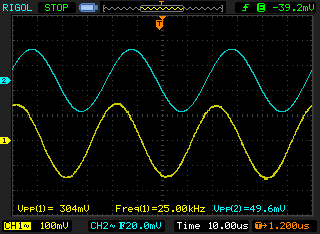
\includegraphics[width=\textwidth]{hpf_osc_25khz.png}
    \caption{Respuesta temporal en banda de paso ($f = 25.0\,\mathrm{kHz}$): entrada $V_{\text{pp}} = 49.6\,\mathrm{mV}$ (cian), salida $V_{\text{pp}} = 304\,\mathrm{mV}$ (amarillo), verificando una ganancia de $A_v = 6.13\,\mathrm{V/V}$ ($+15.75\,\mathrm{dB}$).}
    \label{fig.ej3:osc_25k}
\end{subfigure}
\caption{Relevamiento temporal del filtro pasa-altos MFB de 4to orden en osciloscopio digital.}
\label{fig.ej3:tiempo}
\end{figure}

Las capturas temporales demuestran inequívocamente el funcionamiento del filtro:
\begin{itemize}
    \item A $25.0 \unit{\kilo\hertz}$ (Figura~\ref{fig.ej3:osc_25k}), dentro de la banda de paso plena, la relación
    entre amplitudes es $304 \unit{\milli\volt} / 49.6 \unit{\milli\volt} = 6.13 \unit{\volt\per\volt}$, verificando
    las 6 veces de ganancia de diseño ($+15.75 \unit{\decibel}$).
    \item A $10.87 \unit{\kilo\hertz}$ (Figura~\ref{fig.ej3:osc_11k}), en la frecuencia nominal de
    $11 \unit{\kilo\hertz}$, la ganancia disminuye a $520 \unit{\milli\volt} / 124 \unit{\milli\volt} = 4.19 \unit{\volt\per\volt}$,
    lo que significa una atenuación relativa de $-3.30 \unit{\decibel}$ ($20\log_{10}(4.19/6.13)$),
    en concordancia con la cota $A_{\max} = 3 \unit{\decibel}$ de Chebyshev.
\end{itemize}

\begin{figure}[!ht]
\centering
\begin{subfigure}[t]{0.48\textwidth}
    \centering
    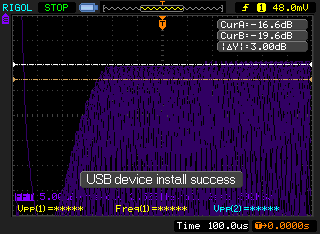
\includegraphics[width=\textwidth]{hpf_fft_mag.png}
    \caption{Espectro FFT del pasa-altos: cursores de amplitud fijados en $\Delta Y = 3.00\,\mathrm{dB}$ ($CurA = -16.6\,\mathrm{dB}$, $CurB = -19.6\,\mathrm{dB}$).}
    \label{fig.ej3:fft_mag}
\end{subfigure}
\hfill
\begin{subfigure}[t]{0.48\textwidth}
    \centering
    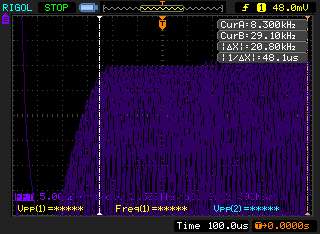
\includegraphics[width=\textwidth]{hpf_fft_freq.png}
    \caption{Espectro FFT del pasa-altos: demarcación de banda y frecuencia de corte con cursores de frecuencia ($CurA = 8.30\,\mathrm{kHz}$, $CurB = 29.10\,\mathrm{kHz}$).}
    \label{fig.ej3:fft_fc}
\end{subfigure}
\caption{Análisis espectral por FFT del filtro pasa-altos MFB en osciloscopio digital.}
\label{fig.ej3:fft}
\end{figure}

El perfil FFT en frecuencia (Figuras~\ref{fig.ej3:fft_mag} y~\ref{fig.ej3:fft_fc}) confirma el comportamiento
pasa-altos de cuarto orden, exhibiendo un rechazo total para bajas frecuencias y una pendiente abrupta en torno a
los $10 \unit{\kilo\hertz}$, validando la exactitud del modelo implementado.

\begin{figure}[!ht]
\centering
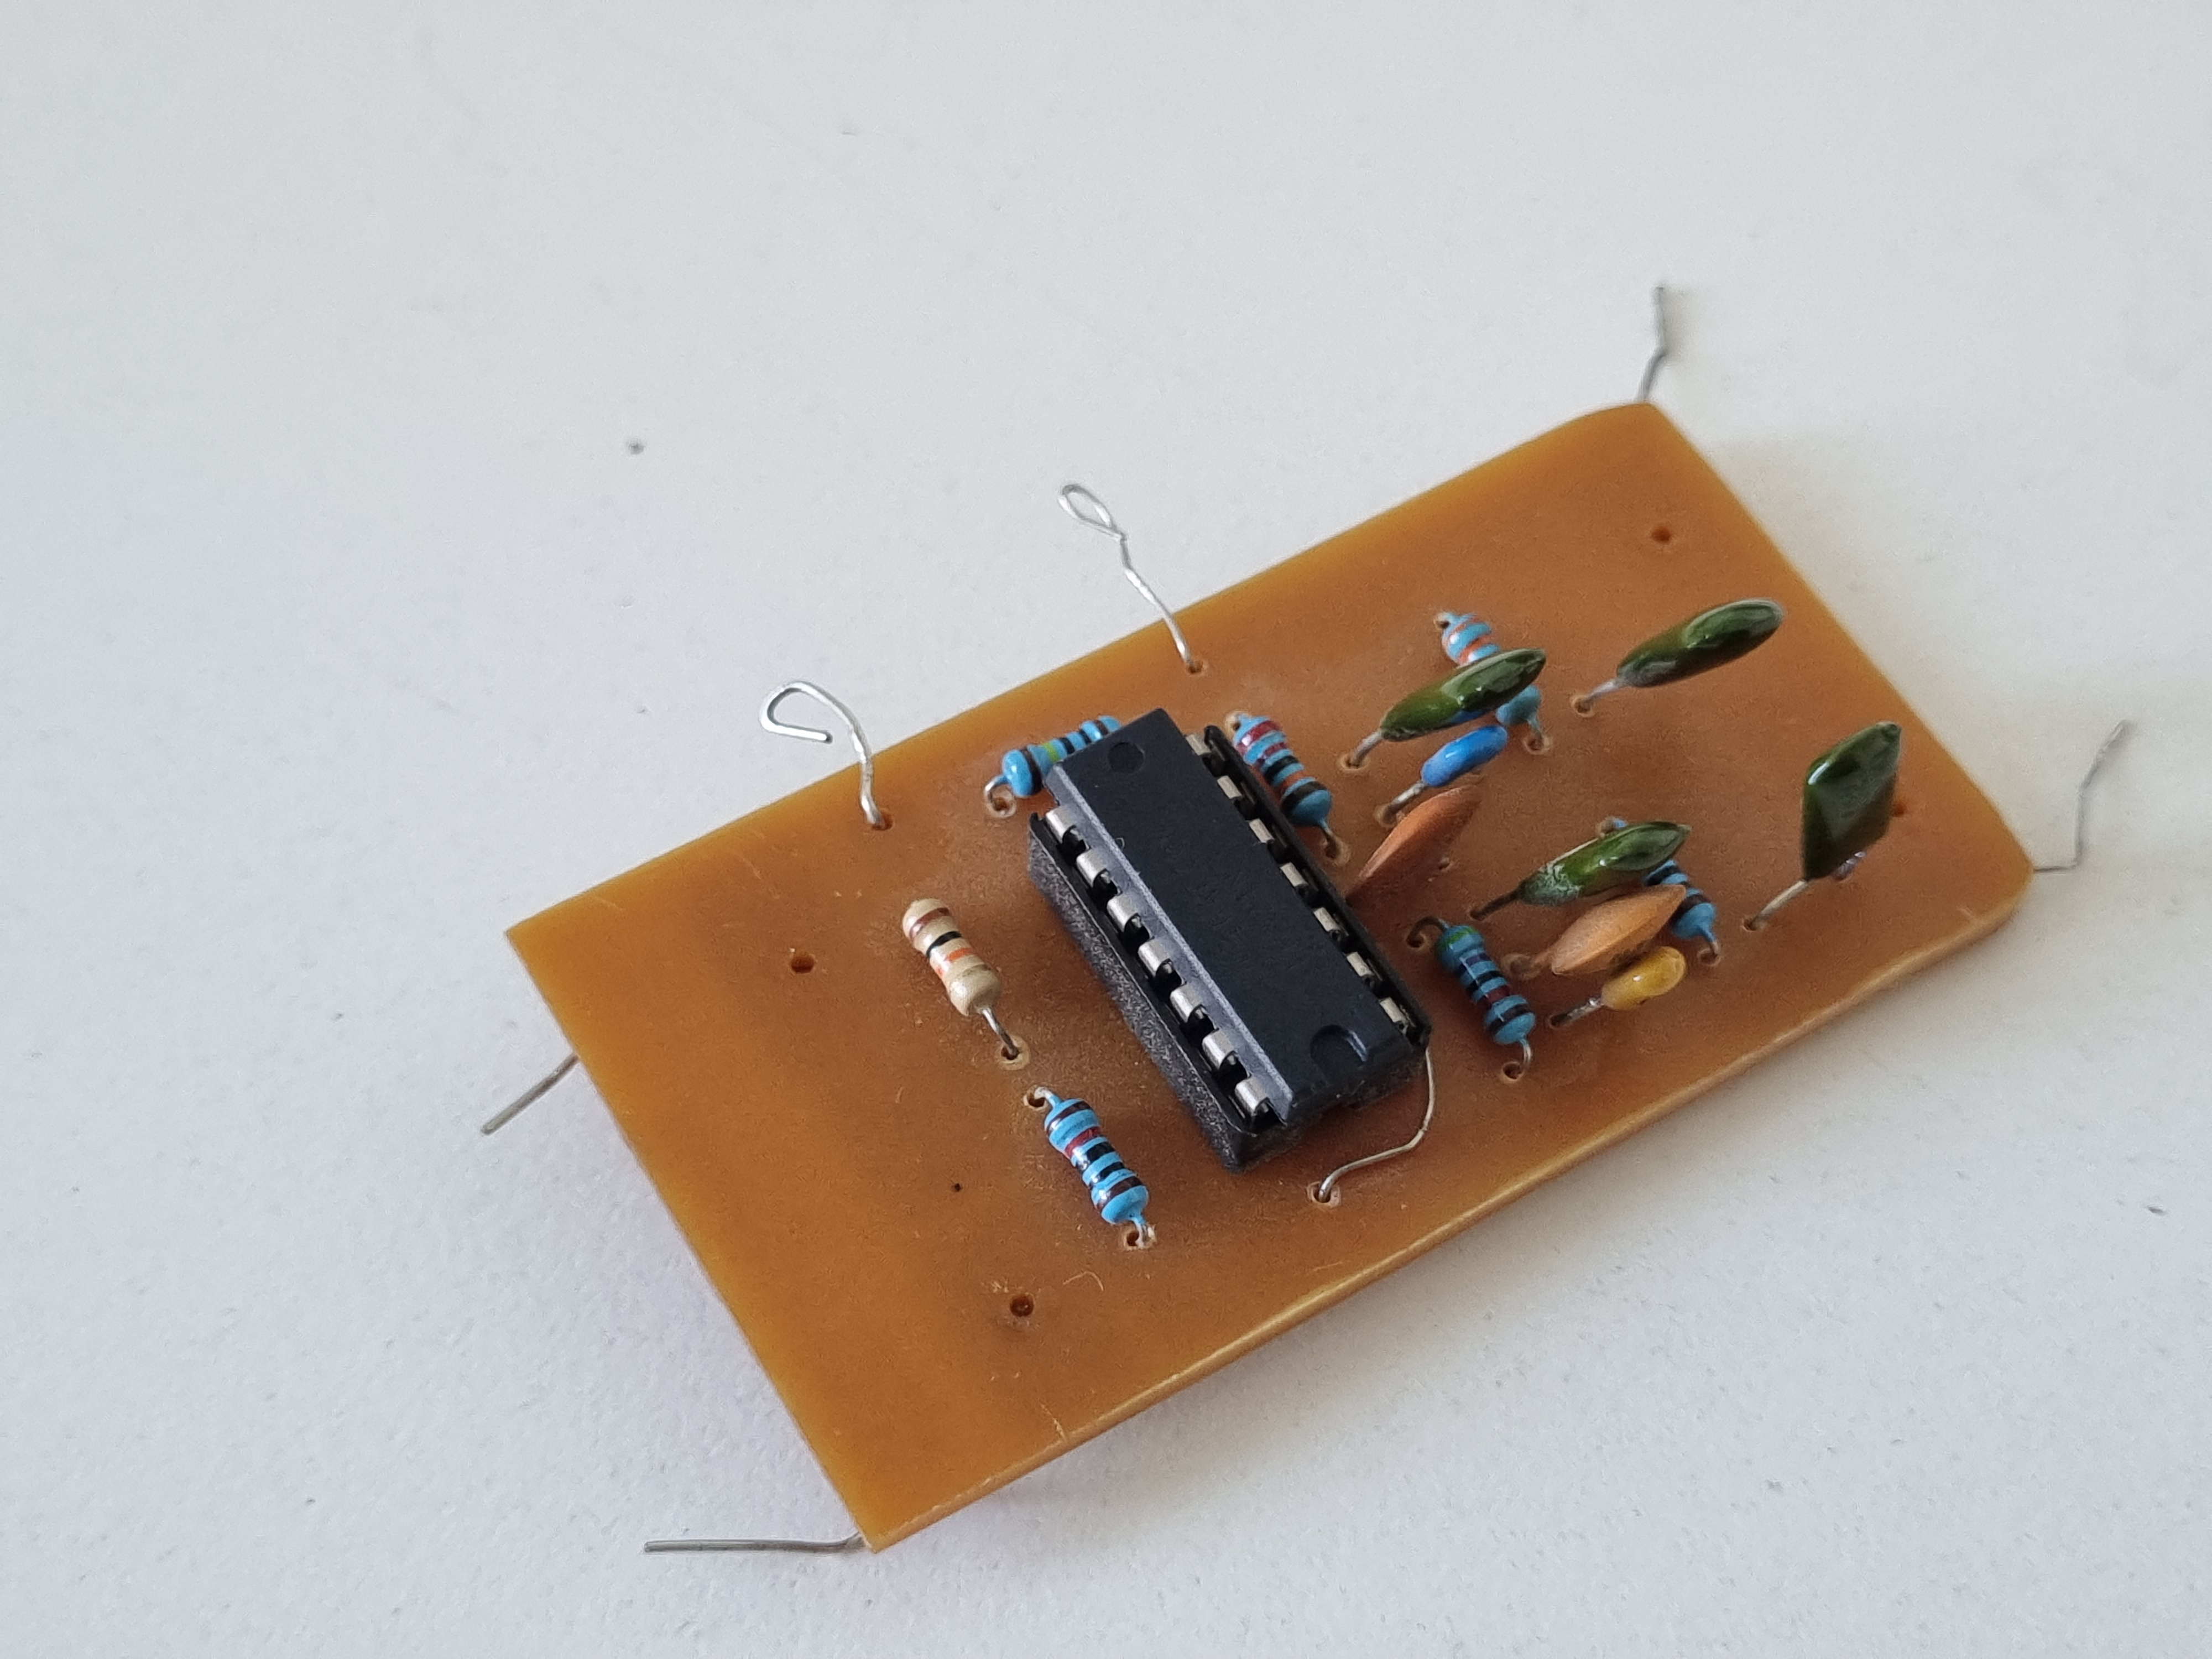
\includegraphics[width=0.68\textwidth]{pcb_hpf_mfb.jpg}
\caption{Placa de circuito impreso implementada para el filtro activo pasa-altos MFB de 4to orden.}
\label{fig.ej3:placa}
\end{figure}
